As mentioned earlier, we wanted to challenge ourselves by writing this paper in \LaTeX{}. \LaTeX{} is based on the markup language TeX, originally developed by the American computer scientist Donald Knuth in 1982. The \LaTeX{} framework used for this project is \dq a macro package built on top of TeX\dq , intended to \dq simplify the typesetting of TeX\dq \footcite{wikibooks_latex_nodate}. Essentially, a \LaTeX{} document is nothing more than a text document enriched with commands and markup.

One of the main differences between \LaTeX{} and conventional text editors such as Microsoft Word is that the author does not immediately see the result of what he is writing. Unlike MS Word, which operates on the principle of WYSIWYG (What You See Is What You Get), \LaTeX{} operates on the principle of WYSIWYAF (What You See Is What You Asked For).

Despite the significant drawback of requiring authors to learn how to use \LaTeX{}, the advantages outweigh the disadvantages. Wikibooks outlines the advantages of \LaTeX{} as follows\footcite{wikibooks_latex_nodate}:
\begin{itemize}
    \item You can concentrate purely on the structure and contents of the document. \LaTeX{} will automatically ensure that the typography of your document—fonts, text sizes, line heights, and other layout considerations—are consistent according to the rules you set.
    \item In \LaTeX{}, the document structure is visible to the user, and can be easily copied to another document. In WYSIWYG applications it is often not obvious how a certain formatting was produced, and it might be impossible to copy it directly for use in another document.
    \item Indexes, footnotes, citations and references are generated easily and automatically.
    \item Mathematical formulae can be easily typeset. (Quality mathematics was one of the original motivations of TeX.)
    \item Since the document source is plain text,
    \item Document sources can be read and understood with any text editor, unlike the complex binary and XML formats used with WYSIWYG programs.
    \item Tables, figures, equations, etc. can be generated programmatically with any language.
    \item Changes can be easily tracked with version control software.
    \item Some academic journals only accept or strongly recommend submissions in the form of \LaTeX{} documents. Publishers offer \LaTeX{} templates.
\end{itemize}

We found these points to be significant advantages in our work with \LaTeX{}, particularly the highly structured approach to document composition and the straightforward handling of sources.

However, a simple \LaTeX{} document would not suffice. The most effective use of \LaTeX{} is to set up an entire \LaTeX{} project, especially when different sections of the paper are written simultaneously by different contributors. Such a \LaTeX{} project allows each part of the structure of the paper, such as chapters including all subchapters, to be divided into individual files. These individual files can then be worked on independently, as they are simply referenced within the existing structure (in our case, from a parent chapter file). This provides the flexibility to create the structure of the whole document without content, and then modify the structure without having to consider the content layout. Furthermore, as mentioned in the advantages of Wikibooks, it is possible to change aspects such as layout and font size centrally.

That is why we decided to take on the challenge of writing this paper in \LaTeX{}. Now we will go into the detailed structure of our \LaTeX{} project.

Fortunately, we were able to adopt the general structure from Andy Grunwald, a former FOM student, who has published a \dq FOM \LaTeX{} template \dq  on GitHub\footcite{grundwald_andygrunwaldfom-latex-template_nodate}. This template has many contributors and is continuously improved and adapted to FOM-specific requirements.

In addition to providing the basic document structure, the template also provides various methods for compiling the associated PDF document for the project. This includes using the provided docker file or the compilation files together with the VS Code extension \dq \LaTeX{} Workshop \dq  by James Yu.

Now let's look at the basic structure of the \LaTeX{} document itself. There is a main file called \dq thesis\_main.tex\dq  which describes the basic configurations for the document, such as font size, font, margins, etc., and defines the structural layout of the thesis. This is done using the \dq \\input{}\dq  method, where the path to the referenced file is enclosed in curly braces. This provides a concise and easy to understand method of defining the structure.

The content chapters are further encapsulated, each having its own \dq structure file\dq  (e.g. chapterOverview.tex). This file references individual chapters, each of which can have its own respective structure. Here is an overview of the structure of the document:

\begin{figure}[H]
    \centering
    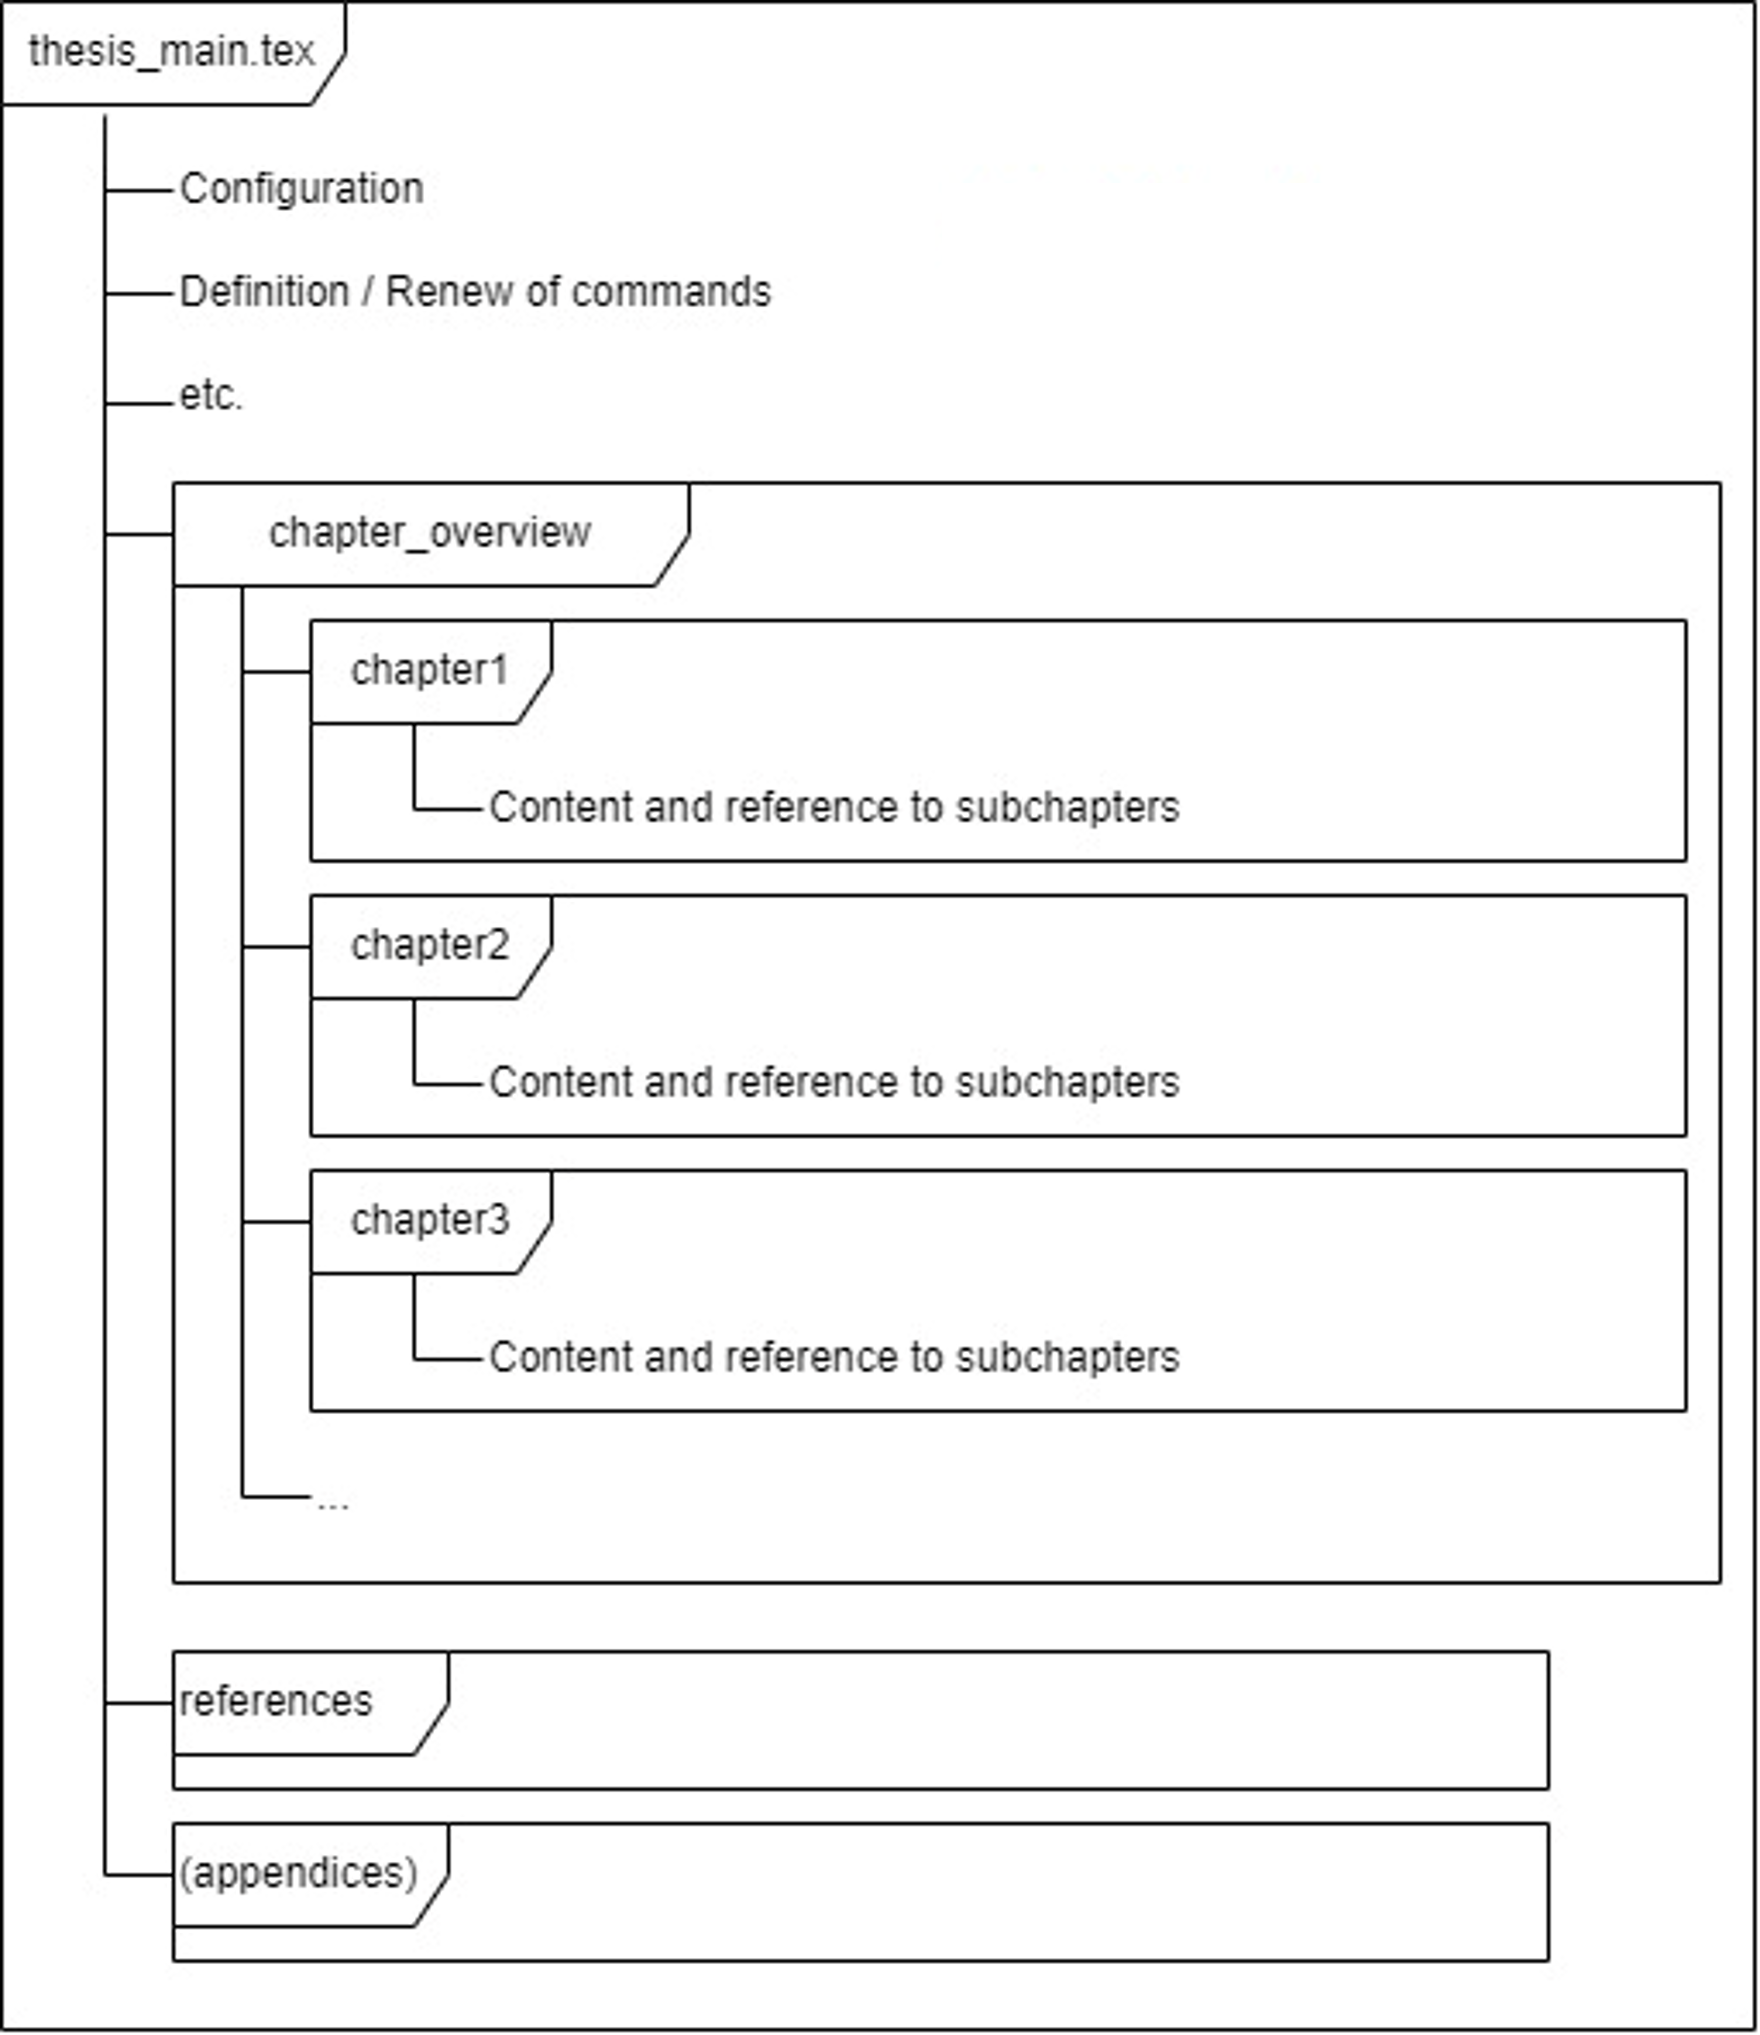
\includegraphics[width=1\textwidth]{filestructure.png}
    \caption{Filestructure, Source: Own depiction}
	\label{fig:filestructure}
\end{figure}

This ensures that the substantive parts (the chapters and subchapters) are separated from the more administrative parts, such as the table of contents. This clear separation is particularly helpful in academic papers where the style, such as numbering, may vary from section to section. With this clear separation, it is possible to apply different styles to each section.

Certainly, other methods would be sufficient for a term project and would achieve similar or identical results. However, as mentioned earlier, we wanted to overcome this technical challenge so that we could use it for future projects.